
RTP transmits the media data over IP using a variety of transport layer
protocols such as UDP, TCP, and Datagram Congestion Control Protocol (DCCP).
Consequetly, congestion control for RTP media flows can be implemented either
in the application or the media flows are transmitted over congestion-
controlled transport (TCP or DCCP). While using a congestion controlled
transport may be safe for the network, it is suboptimal for the media quality
unless the congestion-controlled transport is designed to carry media flows.
On the other hand, using a non-congestion controlled transport (e.g., UDP),
the rate-adaptation is implemented in the application. In this thesis, we
consider congestion control for unicast RTP traffic running over best-effort
IP network. To implement congestion control the sending endpoint needs to rely
on RTCP feedback from the receiver, but unlike other delay-based variants of
TCP there is insufficient RTCP bandwidth to provide feedback on a per-packet
basis.

% CC should not cause queuing delay. Or define low-delay operation of
% multimedia cc.

\section{Framework}
\label{fw.fw}


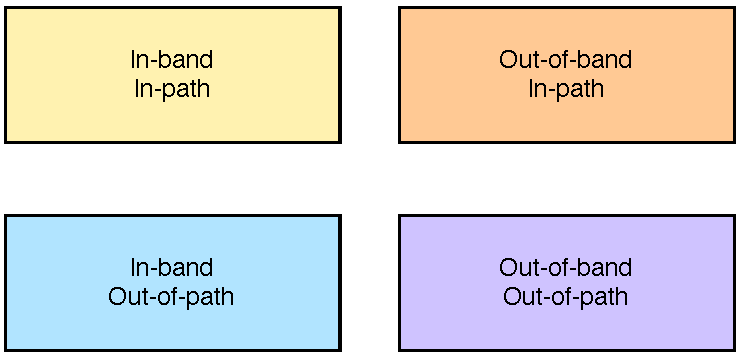
\includegraphics[scale=1.0]{chap2-fw-outline}

\section{Requirements for Congetsion Control}
\label{fw.cc.eval}